\section{Diseño}
\label{s2:sec:Disenyo}

\subsection{Componentes del sistema}
\label{s2:subsec:sistema-entero}
A la hora de realizar el sistema, se ha decidido utilizar los siguientes
componentes:
\begin{itemize}
\item \emph{FGPA}, que como se ha comentado en la sección anterior, es la
  encargada de realizar los cálculos del juego, interpretar las órdenes de
  los usuarios, y mostrar el juego mediante un monitor VGA.
\item \emph{Maletines ARM}, encargados de leer las órdenes de los
  jugadores (mediante pulsaciones en el teclado matricial o los botones de
  la placa) y transmitirlas a la FPGA mediante una UART. Como la FPGA
  utilizada únicamente posee una UART, los maletines se pueden conectar en
  serie, y transmitir los mensajes de uno hacia el siguiente hasta que
  lleguen a la FPGA (ver sección~\ref{s3:subsec:maletines}). Además, la
  FPGA transmite la información de puntuación a los maletines, los cuales
  la muestran mediante sus \emph{Display 8-Segmentos}.
\item \emph{Display 8-Segmentos}, utilizado para mostrar la información de
  puntuación.
\item \emph{Pulsadores y teclado matricial}, para que los jugadores
  indiquen sus órdenes de movimiento al sistema.
\item \emph{Monitor VGA}, utilizado para mostrar el juego.
\end{itemize}

A continuación se muestra tanto el comportamiento global del sistema, como
la comunicación entre los distintos componentes. En la sección siguiente
se muestra con más detalle el funcionamiento del componente FPGA
(apartado~\ref{s3:subsec:fpga}) y de los maletines ARM
(apartado~\ref{s3:subsec:maletines}).

\subsection{Comportamiento del sistema}
\label{s2:subsec:comportamiento}
\todo{Aquí habría que hablar del comportamiento general del sistema, es
  decir, de la máquina de estados que implementa, o de que hace el bicho, o
  de cómo se controla. No se si se podría quizás juntar con la sección
  siguiente y ampliarla, o mejor así. Quizás también se podría aprovechar
  la figura~\ref{s3:fig:FSM_maletin} para mostrarla aquí, aunque faltaría
  todo el tema de la fpga.}\\

\todo{ Quizás lo más fácil es crear una máquina de estados (o red de Petri
  para poder mostrar el paralelismo), y dejarlo tal cual está.}

\begin{figure}[h]
  \centering
  \todo{Poner una FSM, o red de petri, o secuencia, o yo qué sé.}
  
\includegraphics[width=0.5\textwidth]{images/Todo.pdf}
  \caption{Comportamiento del sistema.}
  \label{s2:fig:comportamiento}
\end{figure}

\subsection{Comunicación entre componentes}
\label{s2:subsec:comunicacion}
\rev{Como se ha mencionado anteriormente, el sistema está controlado por
  una FPGA, la cual ejecuta varios bucles de manera paralela para modificar
  el estado del juego y pintar en el monitor VGA los elementos del
  juego}. El resto de componentes (maletín, display 8-Segmentos,
pulsadores, $\ldots$) sirven para modificar el estado del juego mediante
comunicaciones con la FPGA, que permiten que esta calcule las nuevas
posiciones. Según qué componentes interactúen entre ellos, la comunicación
usada es diferente:
\begin{itemize}
\item \emph{FPGA -- VGA:} Comunicación unidireccional utilizando el
  conector VGA. Se utilizan 9 líneas para los colores (3 para cada color),
  y 2 líneas adicionales para la sincronización horizontal y vertical
  respectivamente. \rev{Si da tiempo, el diagrama ?? muestra la máquina de
    estados que controla el dibujado en pantalla.} (Más información se
  puede encontrar en~\cite{Spartan3-StarterKit}).
\item \emph{Pulsadores -- Maletín:} Detección de pulsaciones mediante
  interrupciones en la placa.
\item \emph{Maletín -- Maletín:} Comunicación mediante UARTs. El diseño
  utilizado permite conectar varios maletines en serie, por lo que el
  comportamiento general de los maletines es recibir la información por una
  UART, procesarla y reenviarla por la otra UART. Si la información es
  recibida por la \rev{UART0}, se trata de otro maletín que envía información a la
  FPGA, mientras que si se recibe por la \rev{UART1}, es la FPGA la que envía
  información a los maletines.
\item \emph{FPGA - Maletín:} Comunicación mediante UART. Como la FPGA
  únicamente dispone de un puerto UART, la conexión de los maletines se
  hace en serie, siendo los maletines intermedios encargados de reenviar la
  información en ambos sentidos (hacia la FPGA o hacia el resto de
  maletines).
\end{itemize}

La figura~\ref{s2:fig:secuencia} muestra de manera resumida la comunicación
entre los distintos componentes. Como se puede observar, la FPGA posee dos
grandes bucles\footnote{Más información sobre los bucles de la FPGA, y de
  manera especial sobre los distintos relojes utilizados, se puede encontrar
en~\ref{s3:subsubsec:clocking}.} encargados de calcular el estado del juego, y de pintar en
el monitor. Cuando un jugador pulsa un botón, la información es transmitida
a la FPGA a través de los maletines, modificando el cálculo del estado del
juego. En el caso de que un jugador falle, la FPGA envía información hacia
los maletines para informar de la nueva puntuación.

\begin{figure}[h]
  \centering
  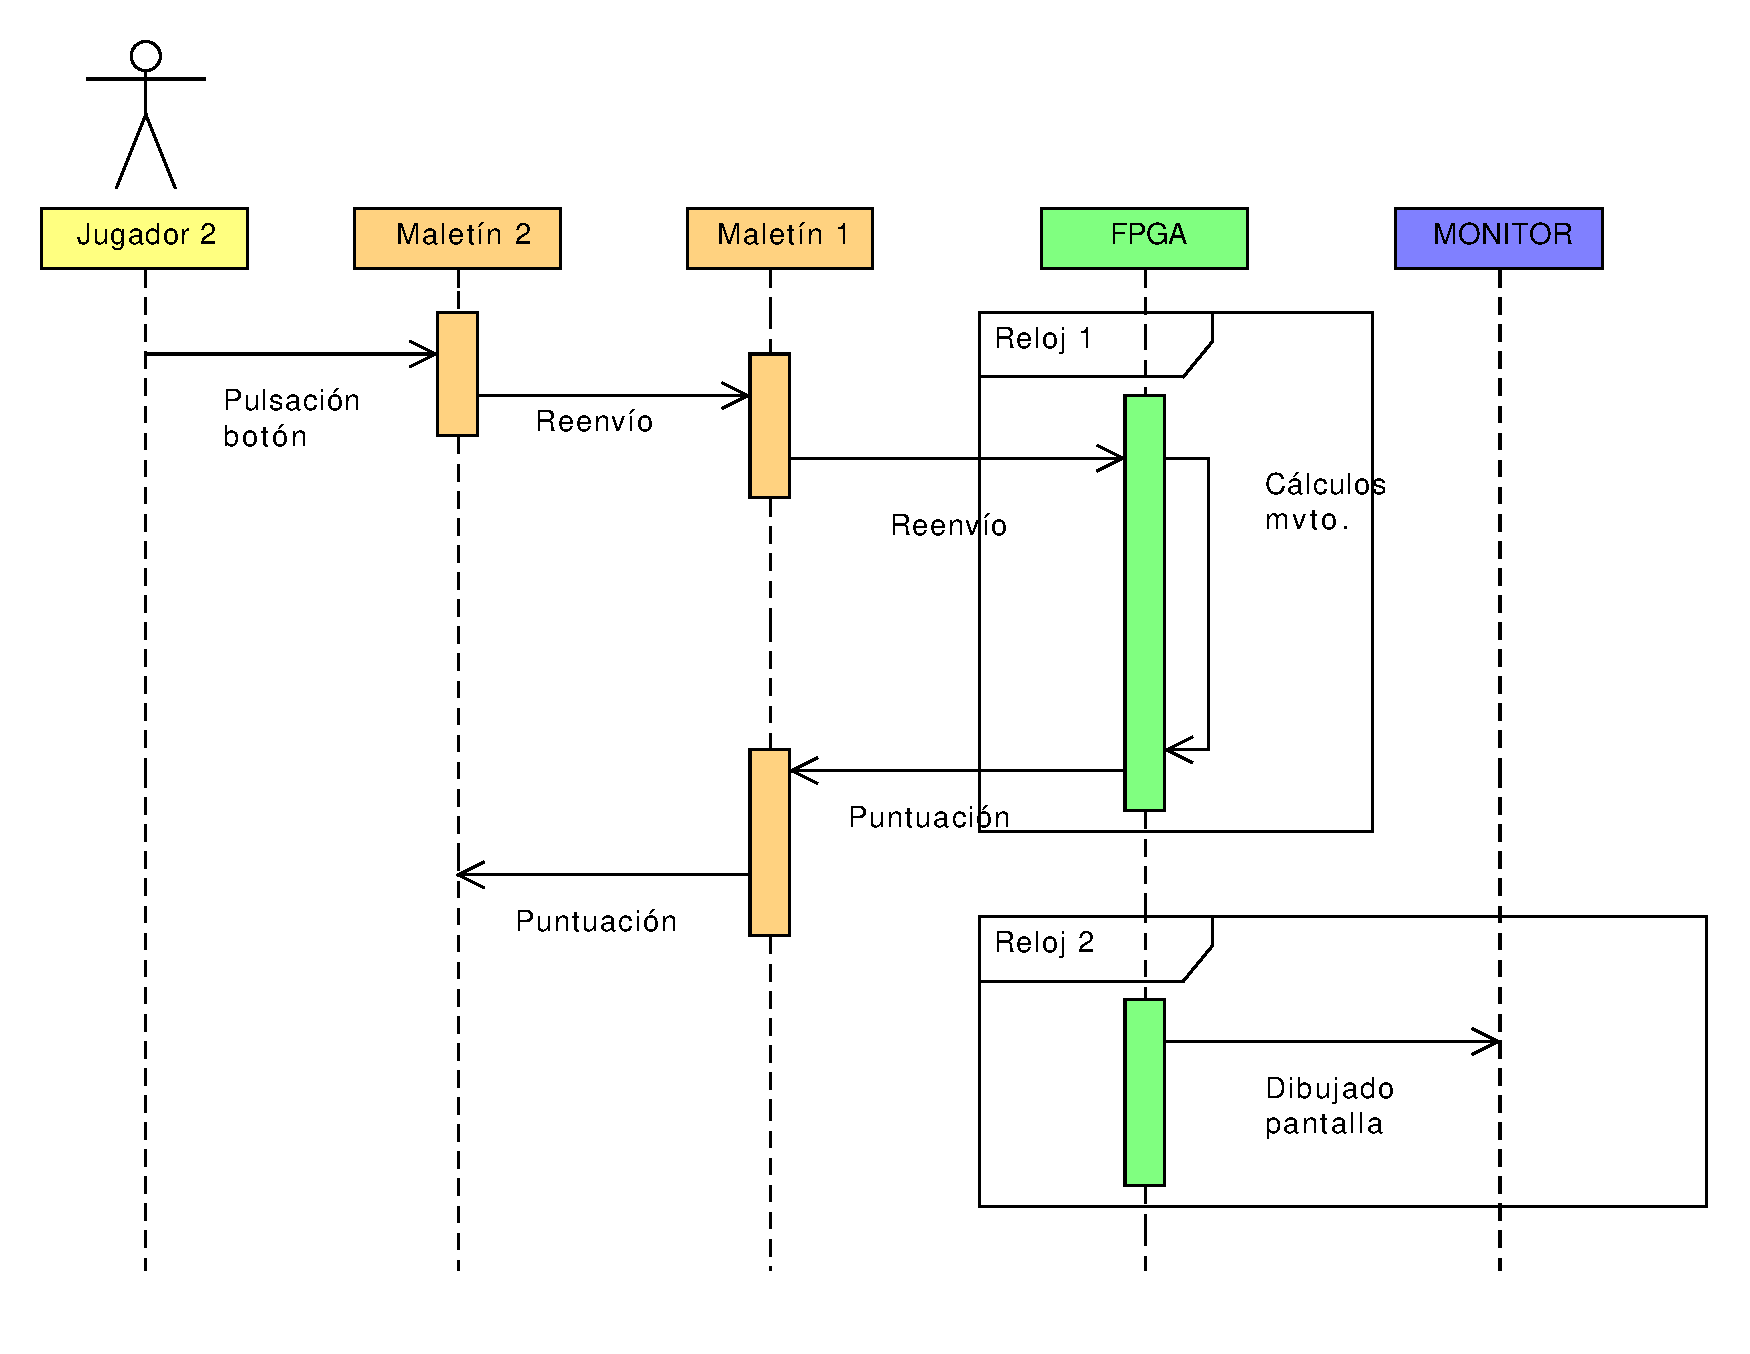
\includegraphics[width=1.0\textwidth]{images/secuencia.pdf}
  \caption{Diagrama de secuencia entre los distintos componentes.}
  \label{s2:fig:secuencia}
p\end{figure}



%
%
%%%
%%% Local Variables:
%%% mode: latex
%%% TeX-master: "../main.tex"
%%% End:


